\documentclass[border=6pt]{standalone}
\usepackage{tikz}
\usetikzlibrary{arrows.meta,positioning,fit,calc}
\definecolor{fg}{HTML}{3B3220}
\definecolor{fgbody}{HTML}{544736}
\definecolor{stroke}{HTML}{7A5A10}
\definecolor{surf}{HTML}{FAF6EE}
\definecolor{surfemph}{HTML}{F2E9D4}
\definecolor{surfact}{HTML}{F6E7E0}
\definecolor{bdim}{HTML}{CFC6B2}
\definecolor{bemph}{HTML}{7A5A10}
\definecolor{bact}{HTML}{8F1D1D}
\begin{document}
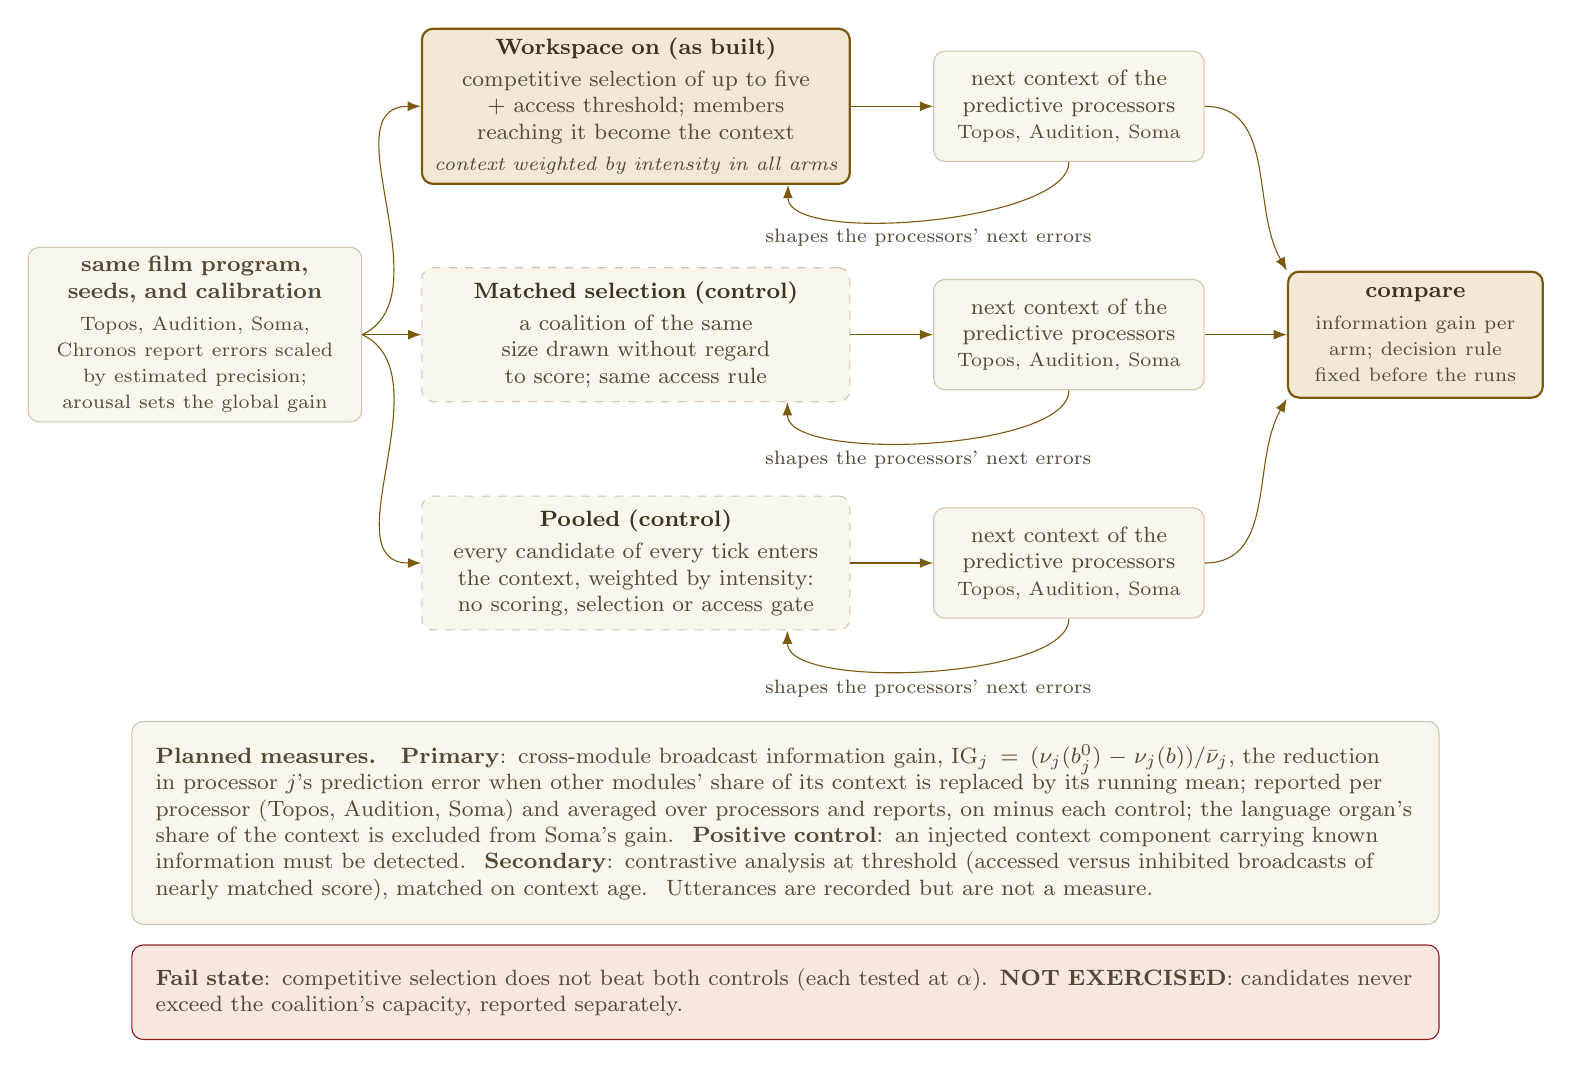
\begin{tikzpicture}[
  font=\small,>=Latex,
  every node/.append style={text=fgbody},
  every node/.append style={execute at begin node={\hyphenpenalty=10000\exhyphenpenalty=10000}},
  mod/.style={draw=bdim, rounded corners, fill=surf, align=center, font=\footnotesize},
  on/.style={draw=bemph, thick, rounded corners, fill=surfemph, align=center, font=\footnotesize},
  off/.style={draw=bdim, dashed, rounded corners, fill=surf, align=center, font=\footnotesize},
  halt/.style={draw=bact, rounded corners, fill=surfact, align=center, font=\footnotesize},
  lbl/.style={font=\footnotesize, text=fgbody, align=center},
]
% shared input
\node[mod, text width=40mm, minimum height=18mm] (shared) at (0,0)
  {\textbf{same film program,\\seeds, and calibration}\\[2pt]\scriptsize Topos, Audition, Soma, Chronos report errors scaled by estimated precision; arousal sets the global gain};
% three arms, in the order of the text
\node[on, text width=52mm, minimum height=17mm] (on) at (5.6,2.9)
  {\textcolor{fg}{\textbf{Workspace on (as built)}}\\[2pt]competitive selection of up to five $+$ access threshold; members reaching it become the context\\[2pt]{\scriptsize\itshape context weighted by intensity in all arms}};
\node[off, text width=52mm, minimum height=17mm] (match) at (5.6,0)
  {\textcolor{fg}{\textbf{Matched selection (control)}}\\[2pt]a coalition of the same size drawn without regard to score; same access rule};
\node[off, text width=52mm, minimum height=17mm] (off) at (5.6,-2.9)
  {\textcolor{fg}{\textbf{Pooled (control)}}\\[2pt]every candidate of every tick enters the context, weighted by intensity: no scoring, selection or access gate};
% context of the predictive processors, one per arm
\node[mod, text width=32mm, minimum height=14mm] (lon) at (11.1,2.9) {next context of the predictive processors\\\scriptsize Topos, Audition, Soma};
\node[mod, text width=32mm, minimum height=14mm] (lmatch) at (11.1,0) {next context of the predictive processors\\\scriptsize Topos, Audition, Soma};
\node[mod, text width=32mm, minimum height=14mm] (loff) at (11.1,-2.9) {next context of the predictive processors\\\scriptsize Topos, Audition, Soma};
% compare
\node[on, text width=30mm, minimum height=16mm] (cmp) at (15.5,0)
  {\textcolor{fg}{\textbf{compare}}\\[2pt]\scriptsize information gain per arm; decision rule fixed before the runs};
% flows
\draw[->, draw=stroke] (shared.east) to[out=25,in=180] (on.west);
\draw[->, draw=stroke] (shared.east) -- (match.west);
\draw[->, draw=stroke] (shared.east) to[out=-25,in=180] (off.west);
\foreach \a/\c in {on/lon, match/lmatch, off/loff} {
  \draw[->, draw=stroke] (\a) -- (\c);
  \draw[->, draw=stroke] (\c.south) to[out=-90,in=-90,looseness=0.55]
    node[lbl, below, font=\scriptsize]{shapes the processors' next errors} ($(\a.south east)+(-8mm,0)$);
}
\draw[->, draw=stroke] (lon.east) to[out=0,in=120] (cmp.north west);
\draw[->, draw=stroke] (lmatch.east) -- (cmp.west);
\draw[->, draw=stroke] (loff.east) to[out=0,in=240] (cmp.south west);
% measures + outcome
\node[mod, text width=160mm, align=left, inner sep=3mm] (meas) at (7.5,-6.2)
  {\textbf{Planned measures.}\;\;
   \textbf{Primary}: cross-module broadcast information gain, $\mathrm{IG}_j=(\nu_j(b^0_j)-\nu_j(b))/\bar\nu_j$, the reduction in processor $j$'s prediction error when other modules' share of its context is replaced by its running mean; reported per processor (Topos, Audition, Soma) and averaged over processors and reports, on minus each control; the language organ's share of the context is excluded from Soma's gain.\;
   \textbf{Positive control}: an injected context component carrying known information must be detected.\;
   \textbf{Secondary}: contrastive analysis at threshold (accessed versus inhibited broadcasts of nearly matched score), matched on context age.\;
   Utterances are recorded but are not a measure.};
\node[halt, text width=160mm, align=left, inner sep=3mm, below=2.5mm of meas] (out)
  {\textbf{Fail state}: competitive selection does not beat both controls (each tested at $\alpha$). \textbf{NOT EXERCISED}: candidates never exceed the coalition's capacity, reported separately.};
\end{tikzpicture}
\end{document}
